\documentclass[tikz,border=0pt]{standalone}
\usepackage{xcolor}
% Palette: Sam_Comm_final.png by eye (as Pursuer's art.py), and Gatecrasher's own.
\definecolor{ink}{HTML}{3B2340}
\definecolor{sky}{HTML}{EFC46A}
\definecolor{skyhi}{HTML}{F5DA92}
\definecolor{skylow}{HTML}{E9B060}
\definecolor{cloud}{HTML}{F2D58A}
\definecolor{wallA}{HTML}{E88A73}
\definecolor{wallB}{HTML}{EE9F7E}
\definecolor{wallC}{HTML}{E47A7E}
\definecolor{wallD}{HTML}{F0B07E}
\definecolor{wallE}{HTML}{D9765F}
\definecolor{wallF}{HTML}{E99A8A}
\definecolor{greenA}{HTML}{8DBB7E}
\definecolor{greenB}{HTML}{6FA77A}
\definecolor{greenC}{HTML}{A9C97F}
\definecolor{greenD}{HTML}{5E9C6A}
\definecolor{window}{HTML}{F6E7A0}
\definecolor{windark}{HTML}{8C5A64}
\definecolor{metal}{HTML}{8D9A93}
\definecolor{metaldark}{HTML}{5E6B66}
\definecolor{wood}{HTML}{B9835A}
\definecolor{paving}{HTML}{E2BD8C}
\definecolor{ground}{HTML}{D3A77D}
\definecolor{stone}{HTML}{E7C9A0}
\definecolor{paper}{HTML}{F6E7C4}
\definecolor{cardboard}{HTML}{C9A06A}
\definecolor{cardboarddark}{HTML}{A47C4C}
\definecolor{red}{HTML}{B3262E}
\definecolor{eyewhite}{HTML}{FBF4E4}
\definecolor{skin}{HTML}{E8B07C}
\definecolor{skinB}{HTML}{C98B5E}
\definecolor{skinC}{HTML}{F2C9A0}
\definecolor{hairdark}{HTML}{2A1E33}
\definecolor{hairred}{HTML}{A8553A}
\definecolor{leather}{HTML}{33293D}
\definecolor{chrome}{HTML}{C9D3CF}
\definecolor{chromedark}{HTML}{7F8C88}
\definecolor{glass}{HTML}{A9D4CB}
\definecolor{lamp}{HTML}{FFE6A3}
\definecolor{smoke}{HTML}{E8D3AE}
\definecolor{shingle}{HTML}{C9604F}
\definecolor{gold}{HTML}{F2B53A}
\definecolor{portalblue}{HTML}{2FA8E8}
\definecolor{portalbluehi}{HTML}{A6DDF5}
\definecolor{portalorange}{HTML}{F2812E}
\definecolor{portalorangehi}{HTML}{F9C891}
\definecolor{olive}{HTML}{7A8450}
\definecolor{olivedark}{HTML}{5C6539}
\definecolor{khaki}{HTML}{C2A66E}
\definecolor{khakidark}{HTML}{9E8350}
\definecolor{mule}{HTML}{9A6A44}
\definecolor{muledark}{HTML}{6B4730}
\definecolor{mulelight}{HTML}{C99A6E}
\definecolor{bandana}{HTML}{C8343A}
\definecolor{suit}{HTML}{56704F}
\definecolor{camoA}{HTML}{8DA867}
\definecolor{camoB}{HTML}{3B5240}
\definecolor{lens}{HTML}{8EF0C6}
\definecolor{lenshi}{HTML}{E2FFF2}
\definecolor{sea}{HTML}{5FB3B0}
\definecolor{seahi}{HTML}{8FCFC0}
\definecolor{seadark}{HTML}{3F8F92}
\definecolor{concrete}{HTML}{E6C29A}
\definecolor{concretedark}{HTML}{C9A07A}
\definecolor{heli}{HTML}{4F8F86}
\definecolor{helidark}{HTML}{3A6C66}
\definecolor{duskA}{HTML}{7A5272}
\definecolor{duskB}{HTML}{B06A78}
\definecolor{duskC}{HTML}{DE8E72}
\definecolor{dirt}{HTML}{C08A68}
\definecolor{dirtdark}{HTML}{A87256}
\definecolor{beam}{HTML}{FFF3BE}
\definecolor{sunA}{HTML}{F3B86A}
\definecolor{sunB}{HTML}{EE9268}
\definecolor{sunC}{HTML}{E57766}
\definecolor{sundisc}{HTML}{FBE3A0}
\definecolor{seadusk}{HTML}{6F9E9C}
\definecolor{balloon}{HTML}{F8F0DE}
\definecolor{hay}{HTML}{E9C46A}
\definecolor{haydark}{HTML}{C99B45}
\definecolor{barn}{HTML}{C9604F}
\definecolor{trim}{HTML}{F6E7C4}
\begin{document}
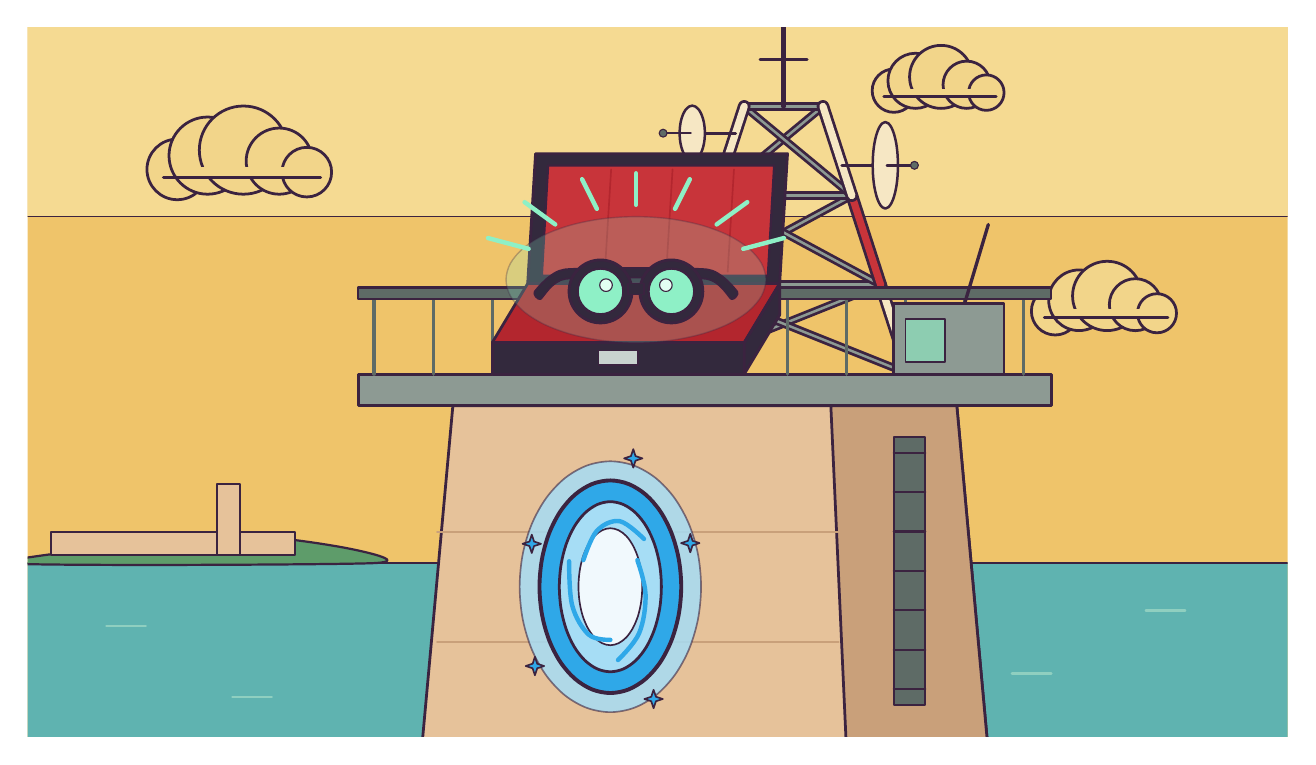
\begin{tikzpicture}
\useasboundingbox (0,0) rectangle (16,9);
\clip (0,0) rectangle (16,9);
\filldraw[draw=ink, line width=1pt, line join=round, fill=sky] (-0.2,-0.2) -- (16.2,-0.2) -- (16.2,9.2) -- (-0.2,9.2) -- cycle;
\filldraw[draw=ink, line width=0.6pt, line join=round, fill=skyhi] (-0.2,6.6) -- (16.2,6.6) -- (16.2,9.2) -- (-0.2,9.2) -- cycle;
\filldraw[draw=ink, line width=1pt, line join=round, fill=sea] (-0.2,-0.2) -- (16.2,-0.2) -- (16.2,2.2) -- (-0.2,2.2) -- cycle;
\draw[seahi, line width=0.9pt, line cap=round, line join=round] (1,1.4) -- (1.5,1.4);
\draw[seahi, line width=0.9pt, line cap=round, line join=round] (12.5,0.8) -- (13,0.8);
\draw[seahi, line width=0.9pt, line cap=round, line join=round] (14.2,1.6) -- (14.7,1.6);
\draw[seahi, line width=0.9pt, line cap=round, line join=round] (2.6,0.5) -- (3.1,0.5);
\filldraw[draw=ink, line width=0.8pt, line join=round, fill=greenD] plot[smooth cycle, tension=0.4] coordinates {(-0.3,2.2) (2.5,2.55) (4,2.4) (4.4,2.2)};
\filldraw[draw=ink, line width=0.7pt, line join=round, fill=concrete] (0.3,2.3) -- (3.4,2.3) -- (3.4,2.6) -- (0.3,2.6) -- cycle;
\filldraw[draw=ink, line width=0.7pt, line join=round, fill=concrete] (2.4,2.3) -- (2.7,2.3) -- (2.7,3.2) -- (2.4,3.2) -- cycle;
\filldraw[draw=ink, line width=1pt, line join=round, fill=cloud] (1.9,7.2) circle (0.385);
\filldraw[draw=ink, line width=1pt, line join=round, fill=cloud] (2.285,7.375) circle (0.49);
\filldraw[draw=ink, line width=1pt, line join=round, fill=cloud] (2.74,7.445) circle (0.56);
\filldraw[draw=ink, line width=1pt, line join=round, fill=cloud] (3.195,7.305) circle (0.42);
\filldraw[draw=ink, line width=1pt, line join=round, fill=cloud] (3.545,7.165) circle (0.315);
\fill[cloud] (1.9,7.095) rectangle (3.545,7.235);
\draw[ink, line width=1.1pt, line cap=round, line join=round] (1.725,7.095) -- (3.72,7.095);
\filldraw[draw=ink, line width=1pt, line join=round, fill=cloud] (13.05,5.4) circle (0.303);
\filldraw[draw=ink, line width=1pt, line join=round, fill=cloud] (13.352,5.538) circle (0.385);
\filldraw[draw=ink, line width=1pt, line join=round, fill=cloud] (13.71,5.593) circle (0.44);
\filldraw[draw=ink, line width=1pt, line join=round, fill=cloud] (14.067,5.482) circle (0.33);
\filldraw[draw=ink, line width=1pt, line join=round, fill=cloud] (14.342,5.373) circle (0.248);
\fill[cloud] (13.05,5.318) rectangle (14.342,5.428);
\draw[ink, line width=1.1pt, line cap=round, line join=round] (12.912,5.318) -- (14.48,5.318);
\filldraw[draw=ink, line width=1pt, line join=round, fill=cloud] (11,8.2) circle (0.275);
\filldraw[draw=ink, line width=1pt, line join=round, fill=cloud] (11.275,8.325) circle (0.35);
\filldraw[draw=ink, line width=1pt, line join=round, fill=cloud] (11.6,8.375) circle (0.4);
\filldraw[draw=ink, line width=1pt, line join=round, fill=cloud] (11.925,8.275) circle (0.3);
\filldraw[draw=ink, line width=1pt, line join=round, fill=cloud] (12.175,8.175) circle (0.225);
\fill[cloud] (11,8.125) rectangle (12.175,8.225);
\draw[ink, line width=1.1pt, line cap=round, line join=round] (10.875,8.125) -- (12.3,8.125);
\draw[ink, line width=2.9pt, line cap=round, line join=round] (8,4.6) -- (10.833,5.733);
\draw[metal, line width=0.9pt, line cap=round, line join=round] (8,4.6) -- (10.833,5.733);
\draw[ink, line width=2.9pt, line cap=round, line join=round] (11.2,4.6) -- (8.367,5.733);
\draw[metal, line width=0.9pt, line cap=round, line join=round] (11.2,4.6) -- (8.367,5.733);
\draw[ink, line width=3.2pt, line cap=round, line join=round] (8.367,5.733) -- (10.833,5.733);
\draw[metal, line width=1.2pt, line cap=round, line join=round] (8.367,5.733) -- (10.833,5.733);
\draw[ink, line width=2.9pt, line cap=round, line join=round] (8.367,5.733) -- (10.467,6.867);
\draw[metal, line width=0.9pt, line cap=round, line join=round] (8.367,5.733) -- (10.467,6.867);
\draw[ink, line width=2.9pt, line cap=round, line join=round] (10.833,5.733) -- (8.733,6.867);
\draw[metal, line width=0.9pt, line cap=round, line join=round] (10.833,5.733) -- (8.733,6.867);
\draw[ink, line width=3.2pt, line cap=round, line join=round] (8.733,6.867) -- (10.467,6.867);
\draw[metal, line width=1.2pt, line cap=round, line join=round] (8.733,6.867) -- (10.467,6.867);
\draw[ink, line width=2.9pt, line cap=round, line join=round] (8.733,6.867) -- (10.1,8);
\draw[metal, line width=0.9pt, line cap=round, line join=round] (8.733,6.867) -- (10.1,8);
\draw[ink, line width=2.9pt, line cap=round, line join=round] (10.467,6.867) -- (9.1,8);
\draw[metal, line width=0.9pt, line cap=round, line join=round] (10.467,6.867) -- (9.1,8);
\draw[ink, line width=3.2pt, line cap=round, line join=round] (9.1,8) -- (10.1,8);
\draw[metal, line width=1.2pt, line cap=round, line join=round] (9.1,8) -- (10.1,8);
\draw[ink, line width=4.6pt, line cap=round, line join=round] (8,4.6) -- (8.367,5.733);
\draw[paper, line width=2.6pt, line cap=round, line join=round] (8,4.6) -- (8.367,5.733);
\draw[ink, line width=4.6pt, line cap=round, line join=round] (8.367,5.733) -- (8.733,6.867);
\draw[bandana, line width=2.6pt, line cap=round, line join=round] (8.367,5.733) -- (8.733,6.867);
\draw[ink, line width=4.6pt, line cap=round, line join=round] (8.733,6.867) -- (9.1,8);
\draw[paper, line width=2.6pt, line cap=round, line join=round] (8.733,6.867) -- (9.1,8);
\draw[ink, line width=4.6pt, line cap=round, line join=round] (11.2,4.6) -- (10.833,5.733);
\draw[paper, line width=2.6pt, line cap=round, line join=round] (11.2,4.6) -- (10.833,5.733);
\draw[ink, line width=4.6pt, line cap=round, line join=round] (10.833,5.733) -- (10.467,6.867);
\draw[bandana, line width=2.6pt, line cap=round, line join=round] (10.833,5.733) -- (10.467,6.867);
\draw[ink, line width=4.6pt, line cap=round, line join=round] (10.467,6.867) -- (10.1,8);
\draw[paper, line width=2.6pt, line cap=round, line join=round] (10.467,6.867) -- (10.1,8);
\draw[ink, line width=1.6pt, line cap=round, line join=round] (9.6,8) -- (9.6,10.2);
\draw[ink, line width=1pt, line cap=round, line join=round] (9.3,8.6) -- (9.9,8.6);
\draw[ink, line width=1pt, line cap=round, line join=round] (9.35,9.1) -- (9.85,9.1);
\draw[ink, line width=1pt, line cap=round, line join=round] (9.4,9.6) -- (9.8,9.6);
\filldraw[draw=ink, line width=0.7pt, line join=round, fill=bandana] (9.6,10.3) circle (0.14);
\draw[ink, line width=1.2pt, line cap=round, line join=round] (10.342,7.252) -- (10.792,7.252);
\filldraw[draw=ink, line width=0.9pt, line join=round, fill=paper] plot[smooth cycle, tension=0.55] coordinates {(11.052,7.252) (11.047,7.394) (11.031,7.527) (11.005,7.641) (10.972,7.728) (10.933,7.783) (10.892,7.802) (10.851,7.783) (10.812,7.728) (10.779,7.641) (10.753,7.527) (10.737,7.394) (10.732,7.252) (10.737,7.11) (10.753,6.977) (10.779,6.863) (10.812,6.776) (10.851,6.721) (10.892,6.702) (10.933,6.721) (10.972,6.776) (11.005,6.863) (11.031,6.977) (11.047,7.11)};
\draw[ink, line width=0.9pt, line cap=round, line join=round] (10.912,7.252) -- (11.242,7.252);
\filldraw[draw=ink, line width=0.4pt, line join=round, fill=metaldark] (11.262,7.252) circle (0.05);
\draw[ink, line width=1.2pt, line cap=round, line join=round] (8.682,6.708) -- (8.232,6.708);
\filldraw[draw=ink, line width=0.9pt, line join=round, fill=paper] plot[smooth cycle, tension=0.55] coordinates {(7.972,6.708) (7.977,6.824) (7.993,6.933) (8.019,7.026) (8.052,7.098) (8.091,7.143) (8.132,7.158) (8.173,7.143) (8.212,7.098) (8.245,7.026) (8.271,6.933) (8.287,6.824) (8.292,6.708) (8.287,6.592) (8.271,6.483) (8.245,6.39) (8.212,6.318) (8.173,6.273) (8.132,6.258) (8.091,6.273) (8.052,6.318) (8.019,6.39) (7.993,6.483) (7.977,6.592)};
\draw[ink, line width=0.9pt, line cap=round, line join=round] (8.112,6.708) -- (7.782,6.708);
\filldraw[draw=ink, line width=0.4pt, line join=round, fill=metaldark] (7.762,6.708) circle (0.05);
\draw[ink, line width=1.2pt, line cap=round, line join=round] (8.99,7.66) -- (8.54,7.66);
\filldraw[draw=ink, line width=0.9pt, line join=round, fill=paper] plot[smooth cycle, tension=0.55] coordinates {(8.28,7.66) (8.285,7.751) (8.301,7.835) (8.327,7.907) (8.36,7.963) (8.399,7.998) (8.44,8.01) (8.481,7.998) (8.52,7.963) (8.553,7.907) (8.579,7.835) (8.595,7.751) (8.6,7.66) (8.595,7.569) (8.579,7.485) (8.553,7.413) (8.52,7.357) (8.481,7.322) (8.44,7.31) (8.399,7.322) (8.36,7.357) (8.327,7.413) (8.301,7.485) (8.285,7.569)};
\draw[ink, line width=0.9pt, line cap=round, line join=round] (8.42,7.66) -- (8.09,7.66);
\filldraw[draw=ink, line width=0.4pt, line join=round, fill=metaldark] (8.07,7.66) circle (0.05);
\filldraw[draw=ink, line width=1pt, line join=round, fill=concrete] (5,-0.2) -- (12.2,-0.2) -- (11.8,4.2) -- (5.4,4.2) -- cycle;
\filldraw[draw=ink, line width=1pt, line join=round, fill=concretedark] (10.4,-0.2) -- (12.2,-0.2) -- (11.8,4.2) -- (10.2,4.2) -- cycle;
\draw[concretedark, line width=0.7pt, line cap=round, line join=round] (5.2,1.2) -- (10.3,1.2);
\draw[concretedark, line width=0.7pt, line cap=round, line join=round] (5.2,2.6) -- (10.3,2.6);
\filldraw[draw=ink, line width=0.6pt, line join=round, fill=portalbluehi, fill opacity=0.85, draw opacity=0.6] plot[smooth cycle, tension=0.55] coordinates {(8.552,1.9) (8.513,2.312) (8.398,2.696) (8.215,3.026) (7.976,3.28) (7.698,3.439) (7.4,3.493) (7.102,3.439) (6.824,3.28) (6.585,3.026) (6.402,2.696) (6.287,2.312) (6.248,1.9) (6.287,1.488) (6.402,1.104) (6.585,0.774) (6.824,0.52) (7.102,0.361) (7.4,0.307) (7.698,0.361) (7.976,0.52) (8.215,0.774) (8.398,1.103) (8.513,1.488)};
\filldraw[draw=ink, line width=1.4pt, line join=round, fill=portalblue] plot[smooth cycle, tension=0.55] coordinates {(8.3,1.9) (8.269,2.249) (8.179,2.575) (8.036,2.855) (7.85,3.069) (7.633,3.204) (7.4,3.25) (7.167,3.204) (6.95,3.069) (6.764,2.855) (6.621,2.575) (6.531,2.249) (6.5,1.9) (6.531,1.551) (6.621,1.225) (6.764,0.945) (6.95,0.731) (7.167,0.596) (7.4,0.55) (7.633,0.596) (7.85,0.731) (8.036,0.945) (8.179,1.225) (8.269,1.551)};
\filldraw[draw=ink, line width=1pt, line join=round, fill=portalbluehi] plot[smooth cycle, tension=0.55] coordinates {(8.048,1.9) (8.026,2.18) (7.961,2.44) (7.858,2.664) (7.724,2.835) (7.568,2.943) (7.4,2.98) (7.232,2.943) (7.076,2.835) (6.942,2.664) (6.839,2.44) (6.774,2.18) (6.752,1.9) (6.774,1.62) (6.839,1.36) (6.942,1.136) (7.076,0.965) (7.232,0.857) (7.4,0.82) (7.568,0.857) (7.724,0.965) (7.858,1.136) (7.961,1.36) (8.026,1.62)};
\filldraw[draw=ink, line width=0.6pt, line join=round, fill=white, fill opacity=0.85] plot[smooth cycle, tension=0.55] coordinates {(7.805,1.9) (7.791,2.092) (7.751,2.271) (7.686,2.425) (7.603,2.543) (7.505,2.617) (7.4,2.643) (7.295,2.617) (7.198,2.543) (7.114,2.425) (7.049,2.271) (7.009,2.092) (6.995,1.9) (7.009,1.708) (7.049,1.529) (7.114,1.375) (7.197,1.257) (7.295,1.183) (7.4,1.157) (7.505,1.183) (7.603,1.257) (7.686,1.375) (7.751,1.529) (7.791,1.708)};
\draw[portalblue, line width=1.6pt, line cap=round, line join=round] plot[smooth, tension=0.6] coordinates {(7.827,2.507) (7.519,2.732) (7.227,2.608) (7.057,2.237)};
\draw[portalblue, line width=1.6pt, line cap=round, line join=round] plot[smooth, tension=0.6] coordinates {(6.876,2.223) (6.916,1.66) (7.126,1.291) (7.4,1.225)};
\draw[portalblue, line width=1.6pt, line cap=round, line join=round] plot[smooth, tension=0.6] coordinates {(7.497,0.969) (7.765,1.309) (7.847,1.801) (7.743,2.237)};
\filldraw[draw=ink, line width=0.6pt, line join=round, fill=portalblue] (8.415,2.571) -- (8.386,2.483) -- (8.298,2.454) -- (8.386,2.425) -- (8.415,2.337) -- (8.444,2.425) -- (8.532,2.454) -- (8.444,2.483) -- cycle;
\filldraw[draw=ink, line width=0.6pt, line join=round, fill=portalblue] (7.691,3.647) -- (7.662,3.559) -- (7.574,3.53) -- (7.662,3.501) -- (7.691,3.413) -- (7.72,3.501) -- (7.808,3.53) -- (7.72,3.559) -- cycle;
\filldraw[draw=ink, line width=0.6pt, line join=round, fill=portalblue] (6.402,2.562) -- (6.373,2.474) -- (6.285,2.445) -- (6.373,2.416) -- (6.402,2.328) -- (6.431,2.416) -- (6.519,2.445) -- (6.431,2.474) -- cycle;
\filldraw[draw=ink, line width=0.6pt, line join=round, fill=portalblue] (6.442,1.01) -- (6.413,0.922) -- (6.325,0.893) -- (6.413,0.864) -- (6.442,0.776) -- (6.471,0.864) -- (6.559,0.893) -- (6.471,0.922) -- cycle;
\filldraw[draw=ink, line width=0.6pt, line join=round, fill=portalblue] (7.949,0.591) -- (7.92,0.503) -- (7.832,0.474) -- (7.92,0.445) -- (7.949,0.357) -- (7.978,0.445) -- (8.066,0.474) -- (7.978,0.503) -- cycle;
\filldraw[draw=ink, line width=0.7pt, line join=round, fill=metaldark] (11,0.4) -- (11.4,0.4) -- (11.4,3.8) -- (11,3.8) -- cycle;
\draw[ink, line width=0.8pt, line cap=round, line join=round] (11,0.6) -- (11.4,0.6);
\draw[ink, line width=0.8pt, line cap=round, line join=round] (11,1.1) -- (11.4,1.1);
\draw[ink, line width=0.8pt, line cap=round, line join=round] (11,1.6) -- (11.4,1.6);
\draw[ink, line width=0.8pt, line cap=round, line join=round] (11,2.1) -- (11.4,2.1);
\draw[ink, line width=0.8pt, line cap=round, line join=round] (11,2.6) -- (11.4,2.6);
\draw[ink, line width=0.8pt, line cap=round, line join=round] (11,3.1) -- (11.4,3.1);
\draw[ink, line width=0.8pt, line cap=round, line join=round] (11,3.6) -- (11.4,3.6);
\filldraw[draw=ink, line width=1pt, line join=round, fill=metal] (4.2,4.2) -- (13,4.2) -- (13,4.6) -- (4.2,4.6) -- cycle;
\draw[metaldark, line width=1.2pt, line cap=round, line join=round] (4.4,4.6) -- (4.4,5.6);
\draw[metaldark, line width=1.2pt, line cap=round, line join=round] (5.15,4.6) -- (5.15,5.6);
\draw[metaldark, line width=1.2pt, line cap=round, line join=round] (5.9,4.6) -- (5.9,5.6);
\draw[metaldark, line width=1.2pt, line cap=round, line join=round] (6.65,4.6) -- (6.65,5.6);
\draw[metaldark, line width=1.2pt, line cap=round, line join=round] (7.4,4.6) -- (7.4,5.6);
\draw[metaldark, line width=1.2pt, line cap=round, line join=round] (8.15,4.6) -- (8.15,5.6);
\draw[metaldark, line width=1.2pt, line cap=round, line join=round] (8.9,4.6) -- (8.9,5.6);
\draw[metaldark, line width=1.2pt, line cap=round, line join=round] (9.65,4.6) -- (9.65,5.6);
\draw[metaldark, line width=1.2pt, line cap=round, line join=round] (10.4,4.6) -- (10.4,5.6);
\draw[metaldark, line width=1.2pt, line cap=round, line join=round] (11.15,4.6) -- (11.15,5.6);
\draw[metaldark, line width=1.2pt, line cap=round, line join=round] (11.9,4.6) -- (11.9,5.6);
\draw[metaldark, line width=1.2pt, line cap=round, line join=round] (12.65,4.6) -- (12.65,5.6);
\filldraw[draw=ink, line width=0.8pt, line join=round, fill=metaldark] (4.2,5.55) -- (13,5.55) -- (13,5.7) -- (4.2,5.7) -- cycle;
\filldraw[draw=ink, line width=1pt, line join=round, fill=leather] (6.35,5.75) -- (9.55,5.75) -- (9.65,7.4) -- (6.45,7.4) -- cycle;
\filldraw[draw=ink, line width=0.8pt, line join=round, fill=bandana] (6.53,5.85) -- (9.4,5.85) -- (9.48,7.25) -- (6.61,7.25) -- cycle;
\draw[red, line width=0.6pt, line cap=round, line join=round] (7.33,5.9) -- (7.41,7.2);
\draw[red, line width=0.6pt, line cap=round, line join=round] (8.11,5.9) -- (8.19,7.2);
\draw[red, line width=0.6pt, line cap=round, line join=round] (8.89,5.9) -- (8.97,7.2);
\filldraw[draw=ink, line width=1pt, line join=round, fill=red] (5.9,5) -- (9.1,5) -- (9.55,5.75) -- (6.35,5.75) -- cycle;
\filldraw[draw=ink, line width=1pt, line join=round, fill=leather] (5.9,5) -- (9.1,5) -- (9.1,4.6) -- (5.9,4.6) -- cycle;
\filldraw[draw=ink, line width=1pt, line join=round, fill=leather] (9.1,4.6) -- (9.55,5.35) -- (9.55,5.75) -- (9.1,5) -- cycle;
\filldraw[draw=ink, line width=0.6pt, line join=round, fill=chrome] (7.25,4.72) -- (7.75,4.72) -- (7.75,4.9) -- (7.25,4.9) -- cycle;
\filldraw[draw=ink, line width=0.5pt, line join=round, fill=lens, fill opacity=0.22, draw opacity=0.3] plot[smooth cycle, tension=0.55] coordinates {(9.375,5.8) (9.319,6.007) (9.154,6.2) (8.892,6.366) (8.55,6.493) (8.152,6.573) (7.725,6.6) (7.298,6.573) (6.9,6.493) (6.558,6.366) (6.296,6.2) (6.131,6.007) (6.075,5.8) (6.131,5.593) (6.296,5.4) (6.558,5.234) (6.9,5.107) (7.298,5.027) (7.725,5) (8.152,5.027) (8.55,5.107) (8.892,5.234) (9.154,5.4) (9.319,5.593)};
\draw[lens, line width=1.6pt, line cap=round, line join=round] (9.088,6.191) -- (9.604,6.328);
\draw[lens, line width=1.6pt, line cap=round, line join=round] (8.75,6.501) -- (9.139,6.784);
\draw[lens, line width=1.6pt, line cap=round, line join=round] (8.221,6.699) -- (8.409,7.075);
\draw[lens, line width=1.6pt, line cap=round, line join=round] (7.725,6.75) -- (7.725,7.15);
\draw[lens, line width=1.6pt, line cap=round, line join=round] (7.229,6.699) -- (7.041,7.075);
\draw[lens, line width=1.6pt, line cap=round, line join=round] (6.7,6.501) -- (6.311,6.784);
\draw[lens, line width=1.6pt, line cap=round, line join=round] (6.362,6.191) -- (5.846,6.328);
\filldraw[draw=ink, line width=0.6pt, line join=round, fill=leather] plot[smooth cycle, tension=0.3] coordinates {(6.438,5.648) (6.818,5.93) (8.632,5.93) (9.012,5.648) (8.938,5.552) (8.618,5.81) (6.832,5.81) (6.512,5.552)};
\filldraw[draw=ink, line width=1pt, line join=round, fill=leather] (7.275,5.65) circle (0.4);
\filldraw[draw=ink, line width=0.8pt, line join=round, fill=lens] (7.275,5.65) circle (0.29);
\filldraw[draw=ink, line width=0.4pt, line join=round, fill=lenshi] (7.345,5.73) circle (0.08);
\filldraw[draw=ink, line width=1pt, line join=round, fill=leather] (8.175,5.65) circle (0.4);
\filldraw[draw=ink, line width=0.8pt, line join=round, fill=lens] (8.175,5.65) circle (0.29);
\filldraw[draw=ink, line width=0.4pt, line join=round, fill=lenshi] (8.105,5.73) circle (0.08);
\filldraw[draw=ink, line width=0.6pt, line join=round, fill=leather] (7.625,5.61) -- (7.825,5.61) -- (7.825,5.75) -- (7.625,5.75) -- cycle;
\filldraw[draw=ink, line width=1pt, line join=round, fill=metal] (11,4.6) -- (12.4,4.6) -- (12.4,5.5) -- (11,5.5) -- cycle;
\filldraw[draw=ink, line width=0.6pt, line join=round, fill=lens, fill opacity=0.6] (11.15,4.75) -- (11.65,4.75) -- (11.65,5.3) -- (11.15,5.3) -- cycle;
\draw[ink, line width=1.2pt, line cap=round, line join=round] (11.9,5.5) -- (12.2,6.5);
\end{tikzpicture}
\end{document}
